\section{Experiments}
\label{sec:experiments}

\subsection{Datasets and Protocols}

We evaluate on two public datasets: AID~\cite{xia2017aid} and NWPU-RESISC45~\cite{cheng2017nwpu}. For each seed, images are shuffled independently within each class, and we then assign 20 images to training, 10 to validation, and all remaining images to testing. The resulting split manifest is stored explicitly and shared by all compared methods under the same seed, so every backbone is trained and evaluated on identical class-balanced partitions. We report the mean and standard deviation over three seeds (3407, 3408, 3409) for all main model comparisons, and the manifest-to-result mapping is retained so that aggregated tables can be regenerated from the same run records.

\subsection{Implementation Details}

Our baseline is ConvNeXt-Tiny~\cite{liu2022convnext}, and the candidate model is the proposed DINOv2-Base adaptive tuning route. All runs use input size $224 \times 224$, AdamW~\cite{loshchilov2019adamw}, cosine learning-rate scheduling, mixed precision, and early stopping based on validation OA. For each backbone family, we keep one training recipe per dataset and reuse it across all three seeds under the same validation protocol, rather than retuning hyperparameters for individual seeds or adjusting settings after observing seed outcomes. The ConvNeXt baseline uses batch size 32, learning rate $1.5\times 10^{-4}$, weight decay 0.05, and up to 80 epochs. The DINOv2 route uses batch size 2 with gradient accumulation 4, learning rate $8\times 10^{-5}$, weight decay 0.01, and up to 60 epochs. For the final DINOv2 setting, we use adapter bottleneck dimension 256, dropout 0.1, gradient checkpointing, unfreezing of only the last transformer block plus final normalization, feature-center loss weight 0.02, and center-update momentum 0.9. To keep component attribution clean, we disable label smoothing, mixup, and cutmix in the final main comparisons. For each run, we record the seed, manifest identifier, configuration snapshot, validation history, OA, AA, Kappa, confusion matrices, class-wise metrics, and reproducible logs.

\subsection{Rebuildable Outputs}

We treat reproducibility artifacts as first-class experimental outputs. For every seed and method, the workflow writes the split manifest, resolved configuration, epoch-wise summaries, prediction artifacts, confusion matrix, and summary metrics. The tables included in this manuscript are rebuilt by aggregation scripts from these recorded outputs rather than by manual transcription. This design matters for geocomputing use: other groups can audit how the reported averages were produced, swap in a different backbone while keeping the same manifests, or reuse the same evaluation chain under related scarce-label protocols.

\subsection{Main Results}

Table~\ref{tab:main_results} reports the three-seed mean and standard deviation of the ConvNeXt baseline and the proposed method under the same seed-controlled data protocol. The proposed route raises mean OA from 0.9179 to 0.9413 on AID and from 0.8721 to 0.8790 on NWPU. The AID result indicates a substantial improvement under the evaluated protocol. The NWPU shift is modest and should be read more cautiously as limited but positive evidence that the workflow remains competitive and stable on a second benchmark, rather than as a large cross-dataset margin. Because the baseline belongs to a different backbone family, Tables~\ref{tab:aid-low20_ablation},~\ref{tab:nwpu-low20_ablation}, and~\ref{tab:stability_results} also report same-backbone controls to separate representation transfer from the contribution of individual adaptation components.

\begin{table}[t]
  \centering
  \scriptsize
  \setlength{\tabcolsep}{2pt}
  \caption{Three-seed mean$\pm$std results under the fixed 20-training and 10-validation images-per-class protocol. $\Delta$OA is measured against the ConvNeXt-Tiny baseline on the same split manifests.}
  \label{tab:main_results}
  \begin{tabular}{l >{\raggedright\arraybackslash}p{0.22\textwidth} c c c c}
    \toprule
    Dataset & Method & OA & AA & Kappa & $\Delta$OA \\
    \midrule
    AID & ConvNeXt-Tiny & 0.9179 $\pm$ 0.0086 & 0.9158 $\pm$ 0.0076 & 0.9150 $\pm$ 0.0089 & -- \\
    AID & DINOv2-B (Adapter, FT) & 0.9413 $\pm$ 0.0036 & 0.9388 $\pm$ 0.0036 & 0.9392 $\pm$ 0.0037 & +0.0234 \\
    NWPU & ConvNeXt-Tiny & 0.8721 $\pm$ 0.0116 & 0.8721 $\pm$ 0.0116 & 0.8691 $\pm$ 0.0119 & -- \\
    NWPU & DINOv2-B (Adapter, FT) & 0.8790 $\pm$ 0.0085 & 0.8790 $\pm$ 0.0085 & 0.8762 $\pm$ 0.0087 & +0.0069 \\
    \bottomrule
  \end{tabular}
\end{table}


Figures~\ref{fig:aid_confusion} and~\ref{fig:nwpu_confusion} show the seed-3407 test-set confusion matrices as illustrative qualitative evidence. Relative to the ConvNeXt-Tiny baseline, the proposed method shows a clearer diagonal concentration on AID and a milder shift on NWPU, which is broadly consistent with the larger quantitative gain on AID and the smaller but still positive mean gain on NWPU. We do not treat these figures as standalone evidence beyond the matched-split comparison shown here.

\begin{figure}[t]
  \centering
  \begin{minipage}{0.48\linewidth}
    \centering
    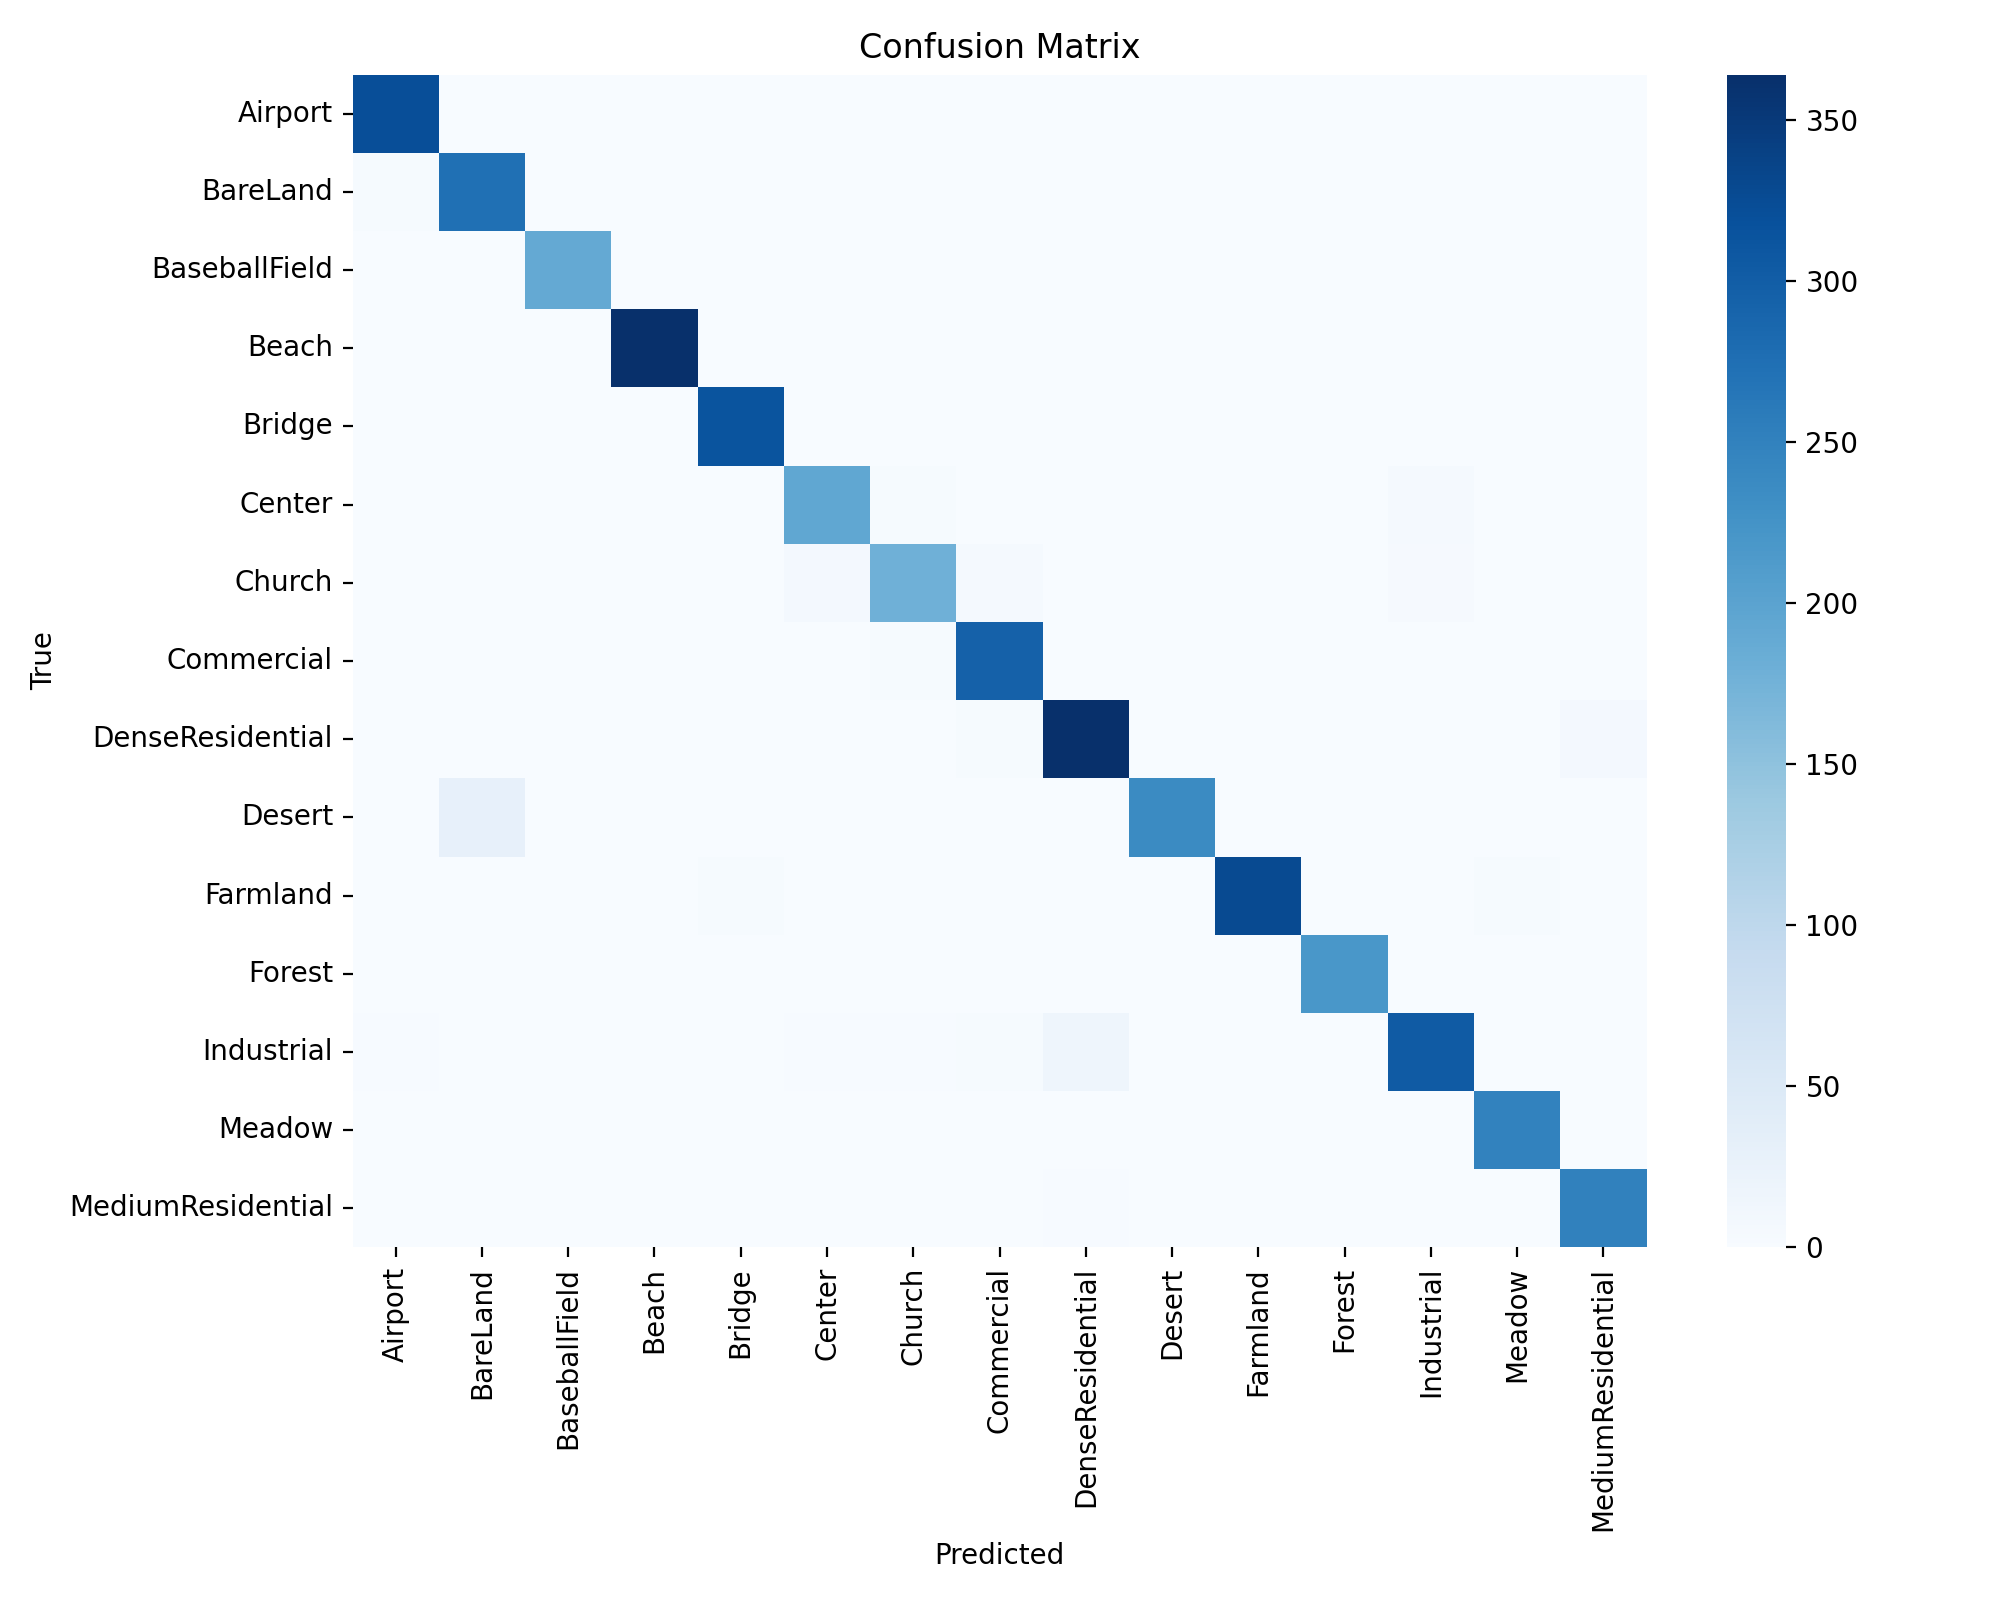
\includegraphics[width=\linewidth]{figures/aid_low20_baseline_confusion.png}
    \par\small (a) ConvNeXt-Tiny baseline
  \end{minipage}\hfill
  \begin{minipage}{0.48\linewidth}
    \centering
    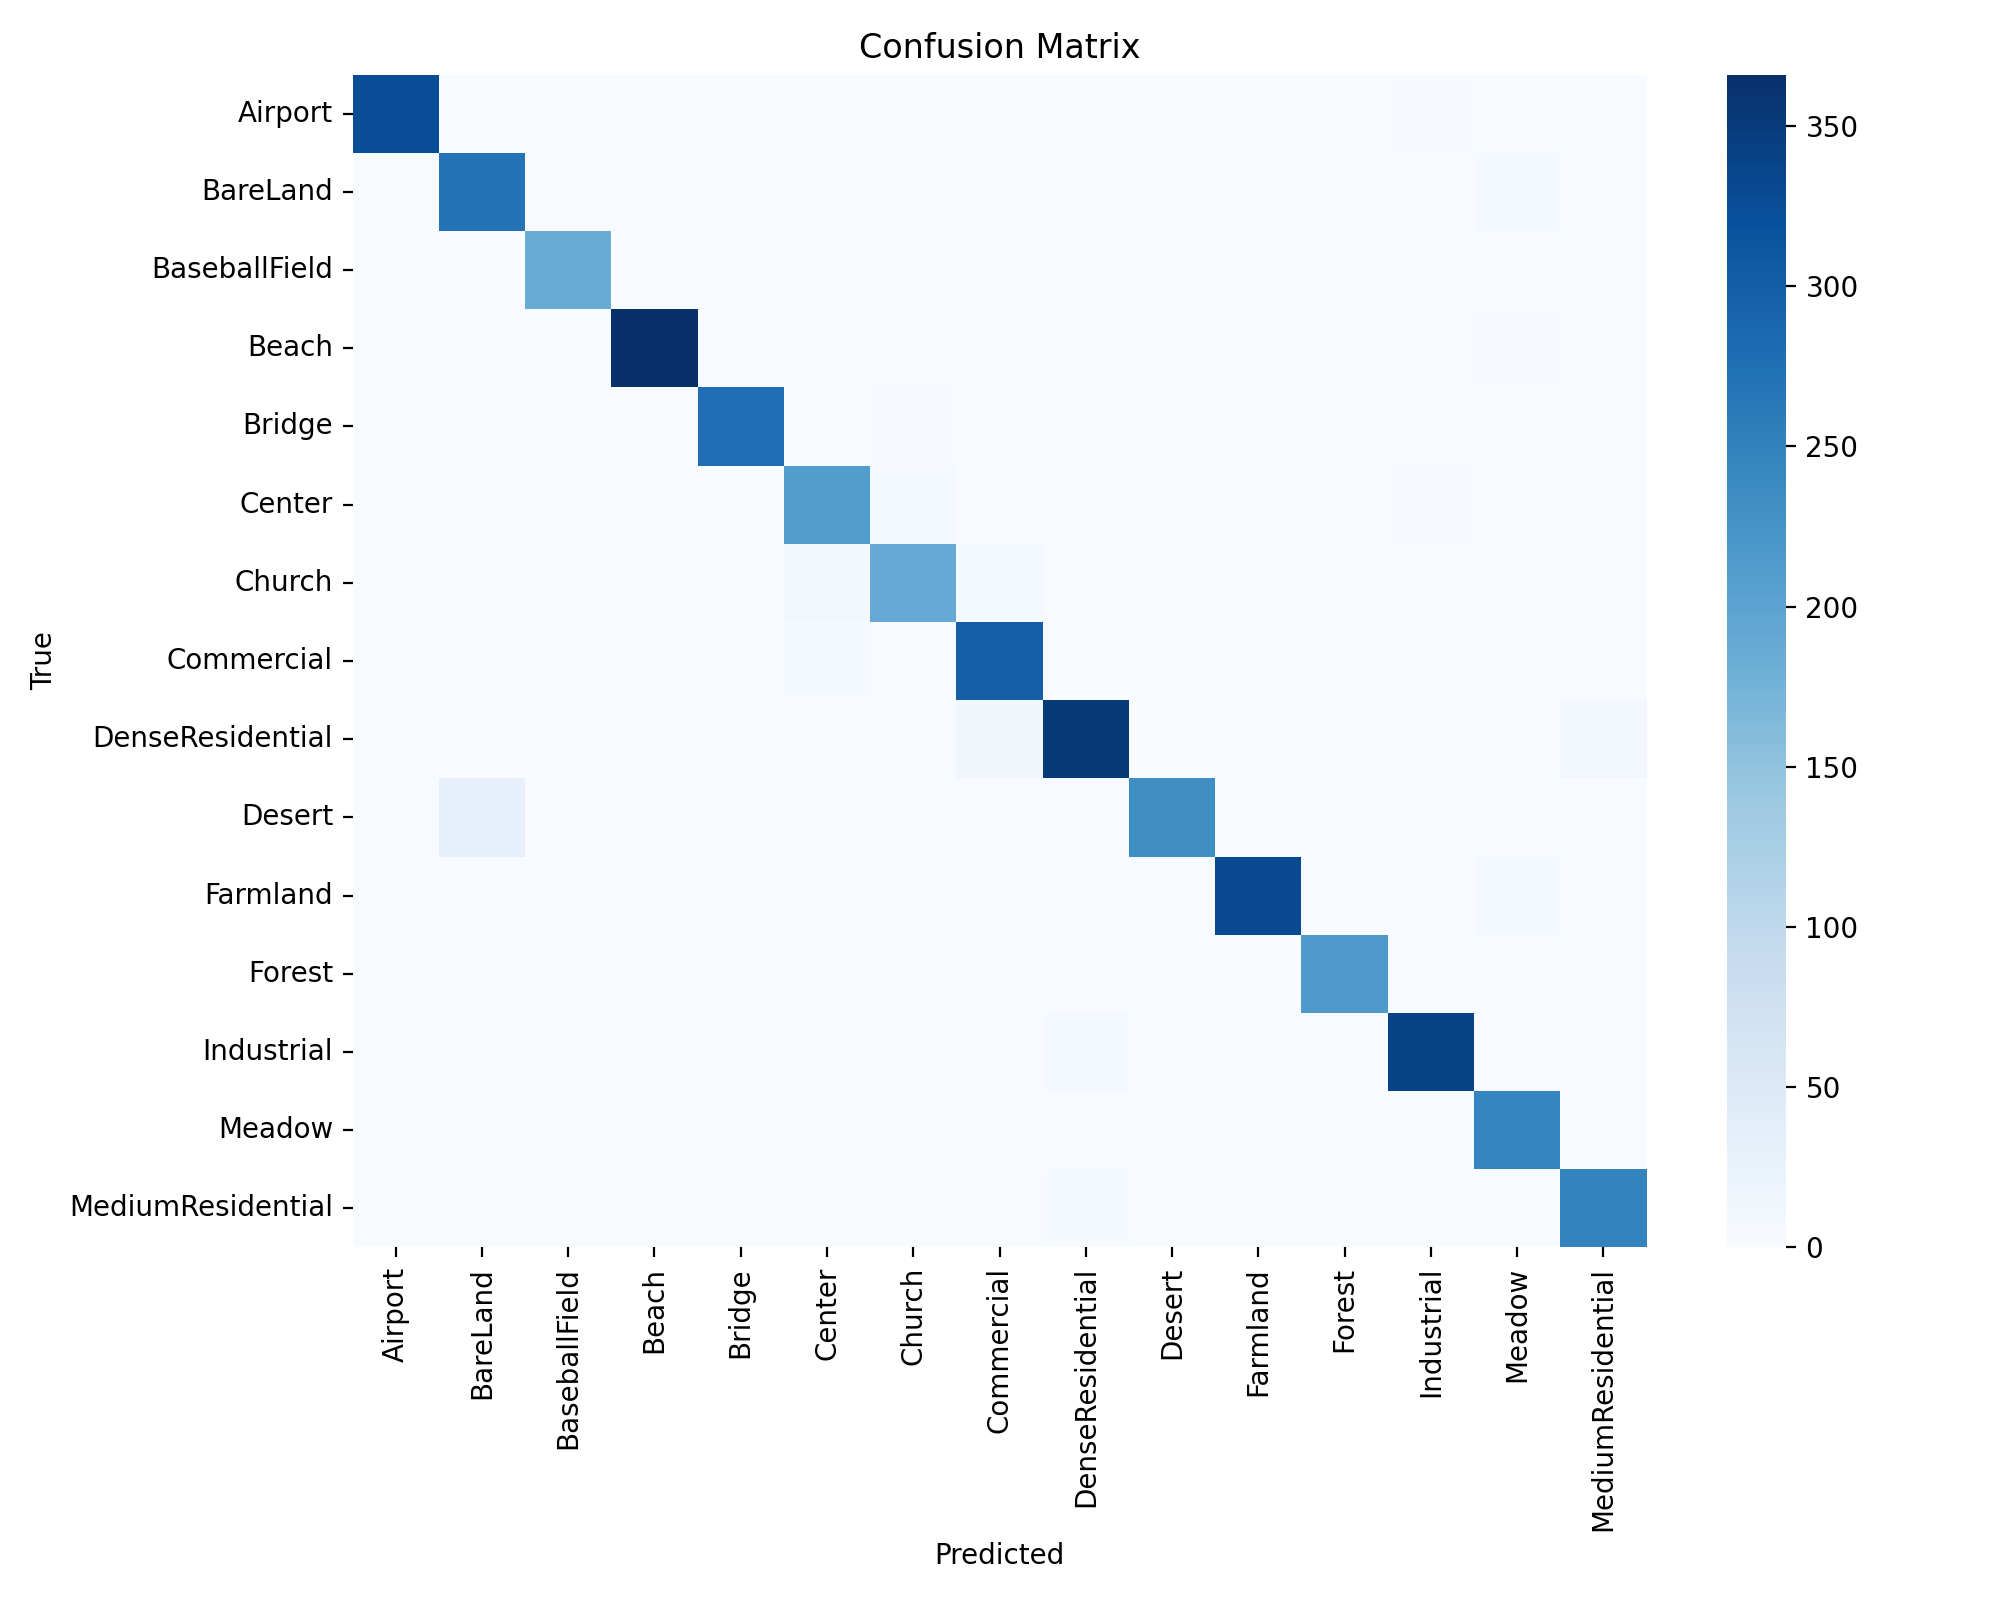
\includegraphics[width=\linewidth]{figures/aid_low20_full_confusion.png}
    \par\small (b) Proposed method
  \end{minipage}
  \caption{Confusion matrices on AID-low20 from seed 3407. Both subfigures use the same test partition, identical class ordering, and the same color scale.}
  \label{fig:aid_confusion}
\end{figure}

\begin{figure}[t]
  \centering
  \begin{minipage}{0.48\linewidth}
    \centering
    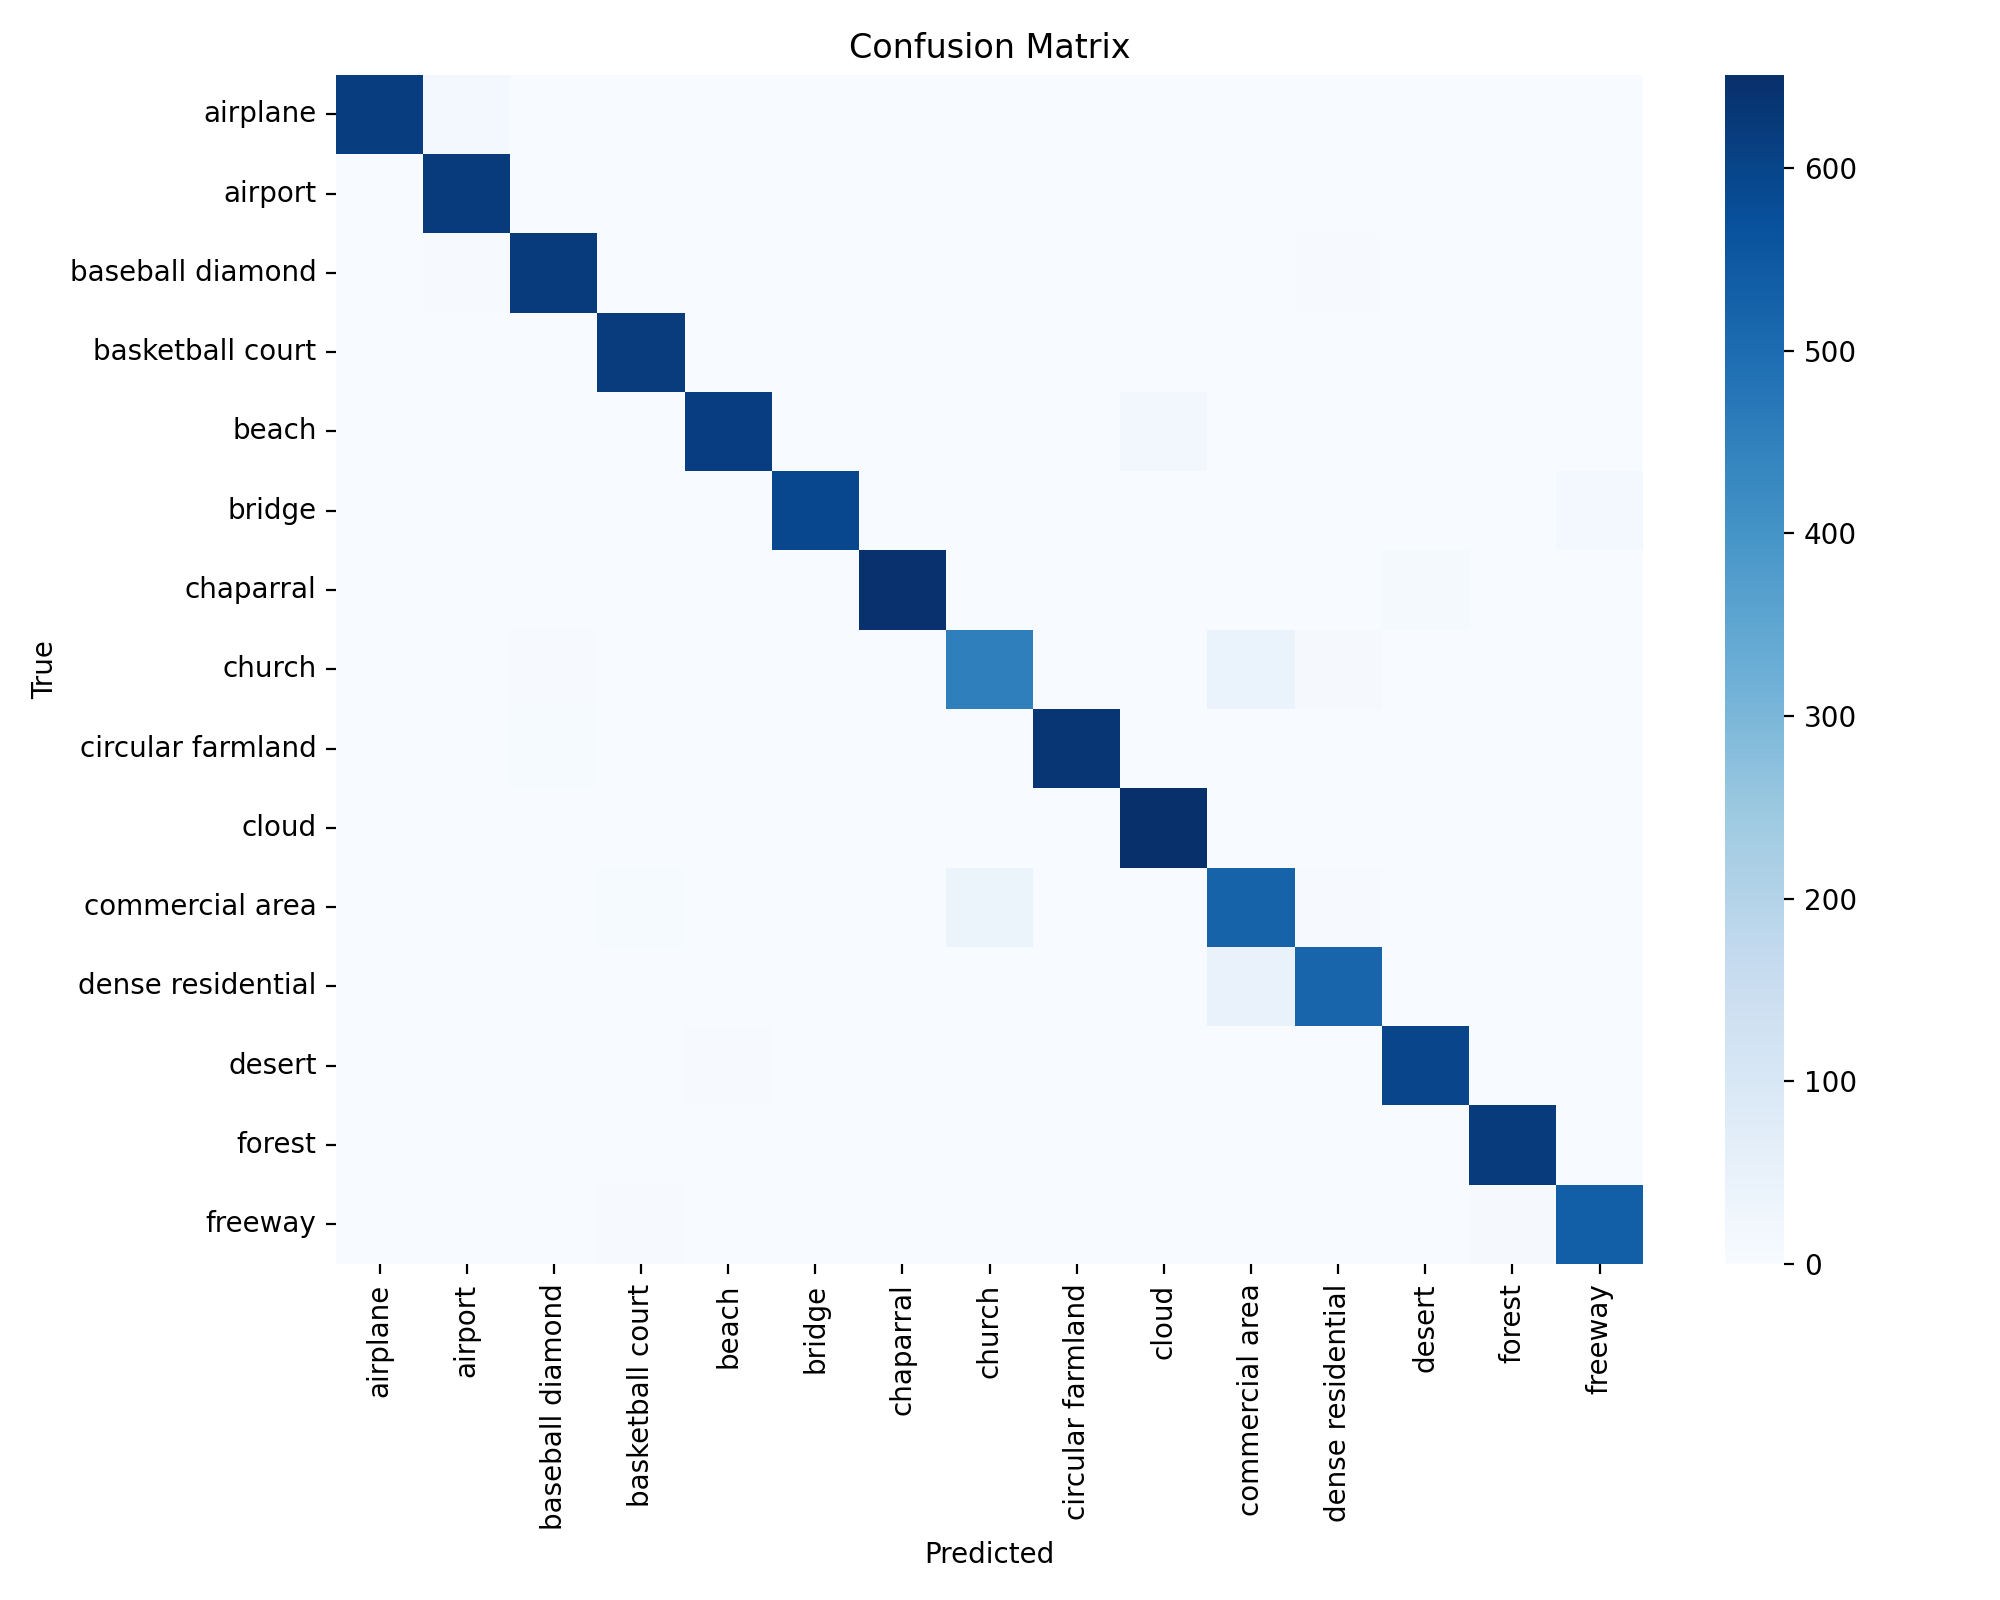
\includegraphics[width=\linewidth]{figures/nwpu_low20_baseline_confusion.png}
    \par\small (a) ConvNeXt-Tiny baseline
  \end{minipage}\hfill
  \begin{minipage}{0.48\linewidth}
    \centering
    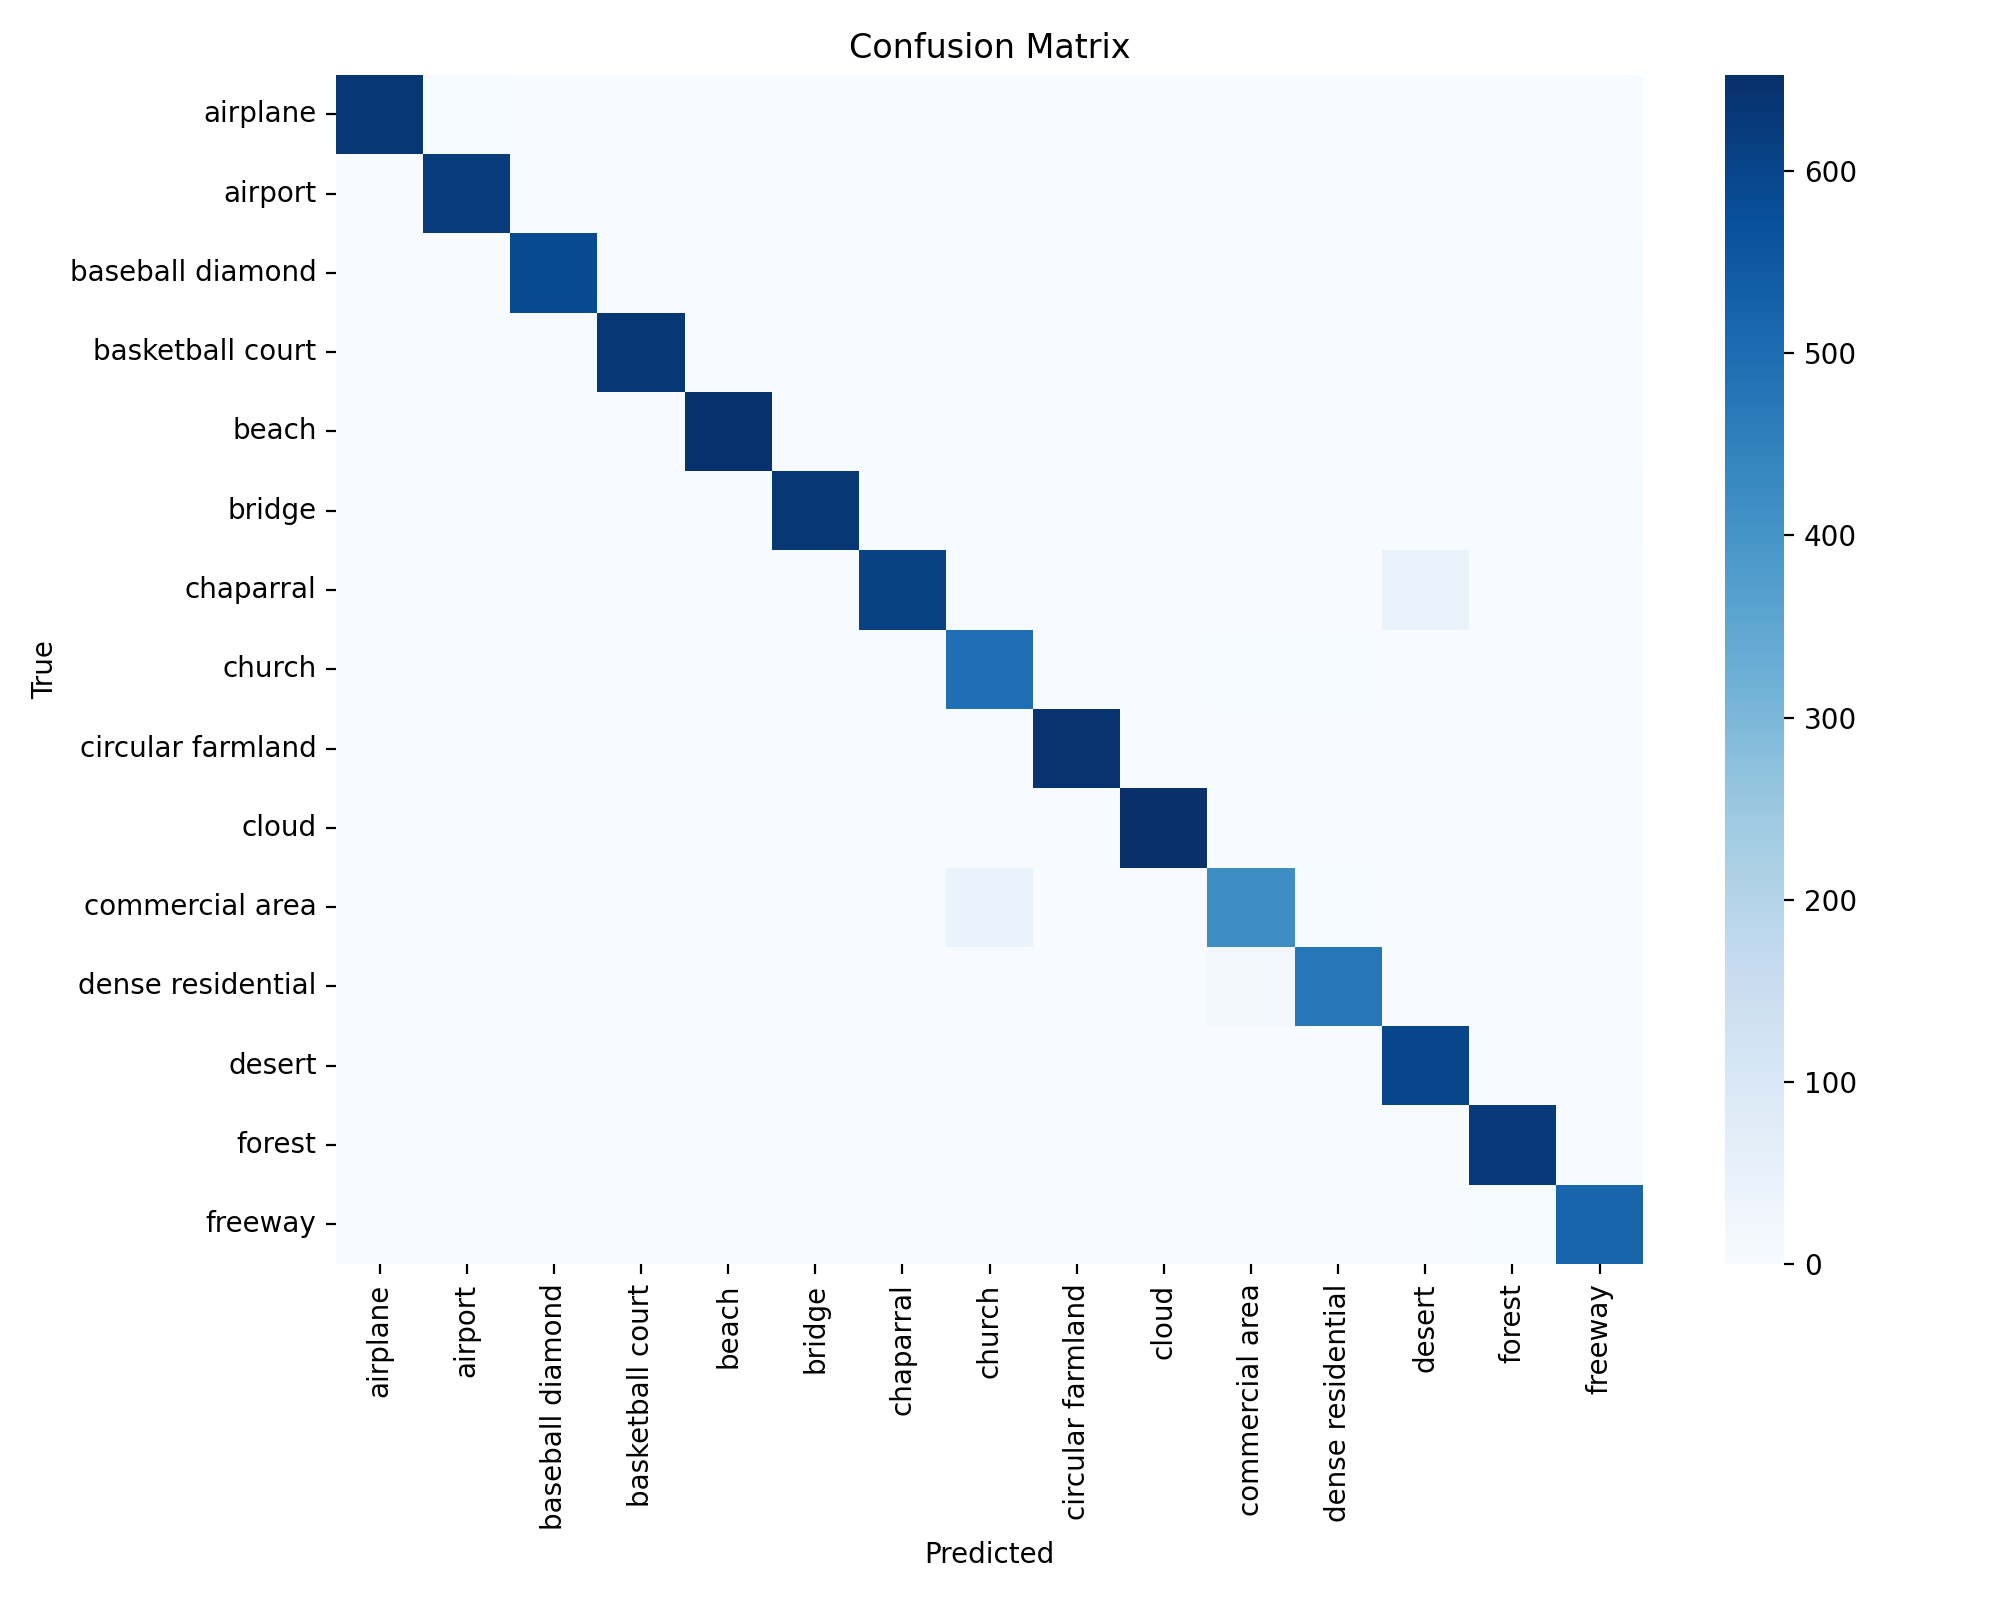
\includegraphics[width=\linewidth]{figures/nwpu_low20_full_confusion.png}
    \par\small (b) Proposed method
  \end{minipage}
  \caption{Confusion matrices on NWPU-low20 from seed 3407. Both subfigures use the same test partition, identical class ordering, and the same color scale.}
  \label{fig:nwpu_confusion}
\end{figure}

\subsection{Ablation Study}

We evaluate variants by removing one component at a time from the main DINOv2 setting. Tables~\ref{tab:aid-low20_ablation} and~\ref{tab:nwpu-low20_ablation} summarize the resulting three-seed ablations:
\begin{itemize}[leftmargin=1.5em]
  \item disabling partial finetuning (adapter-only) causes large degradation on both datasets;
  \item removing the adapter yields very similar mean OA on both datasets (AID: 0.9416 vs 0.9413, NWPU: 0.8793 vs 0.8790), but with larger seed variance than the full setting;
  \item removing feature-center regularization underperforms the full setting on both datasets in three-seed aggregation (AID: 0.9350 vs 0.9413, NWPU: 0.8722 vs 0.8790).
\end{itemize}
These results suggest that selective backbone finetuning contributes most of the mean improvement under the current protocol. The adapter mainly affects robustness and stability, whereas feature-center regularization shows a clear mean benefit on AID and a smaller positive shift on NWPU in three-seed aggregation. All key ablations are therefore reported with complete three-seed evidence. In particular, adapter-only drops to 0.8981 $\pm$ 0.0050 on AID and 0.7782 $\pm$ 0.0369 on NWPU, both below the full method (0.9413 and 0.8790, respectively), which supports keeping partial backbone finetuning in the final configuration under the current protocol. This same-backbone evidence also helps show that the final gains are not explained solely by switching from ConvNeXt to DINOv2; the controlled adaptation design within the DINOv2 route also contributes.

\begin{table}[t]
  \centering
  \caption{Three-seed mean$\pm$std ablation results on AID-low20 under the fixed split protocol.}
  \label{tab:aid-low20_ablation}
  \begin{tabular}{l c c c}
    \toprule
    Variant & OA & AA & Kappa \\
    \midrule
    ConvNeXt-Tiny & 0.9179 $\pm$ 0.0086 & 0.9158 $\pm$ 0.0076 & 0.9150 $\pm$ 0.0089 \\
    NoCenter & 0.9350 $\pm$ 0.0075 & 0.9333 $\pm$ 0.0063 & 0.9327 $\pm$ 0.0078 \\
    NoAdapter & 0.9416 $\pm$ 0.0066 & 0.9391 $\pm$ 0.0067 & 0.9396 $\pm$ 0.0069 \\
    Adapter only & 0.8981 $\pm$ 0.0050 & 0.8969 $\pm$ 0.0044 & 0.8944 $\pm$ 0.0052 \\
    DINOv2-B (Adapter, FT) & 0.9413 $\pm$ 0.0036 & 0.9388 $\pm$ 0.0036 & 0.9392 $\pm$ 0.0037 \\
    \bottomrule
  \end{tabular}
\end{table}

\begin{table}[t]
  \centering
  \caption{Three-seed mean$\pm$std ablation results on NWPU-low20 under the fixed split protocol.}
  \label{tab:nwpu-low20_ablation}
  \begin{tabular}{l c c c}
    \toprule
    Variant & OA & AA & Kappa \\
    \midrule
    ConvNeXt-Tiny & 0.8721 $\pm$ 0.0116 & 0.8721 $\pm$ 0.0116 & 0.8691 $\pm$ 0.0119 \\
    NoCenter & 0.8722 $\pm$ 0.0056 & 0.8722 $\pm$ 0.0056 & 0.8693 $\pm$ 0.0057 \\
    NoAdapter & 0.8793 $\pm$ 0.0112 & 0.8793 $\pm$ 0.0112 & 0.8765 $\pm$ 0.0115 \\
    Adapter only & 0.7782 $\pm$ 0.0369 & 0.7782 $\pm$ 0.0369 & 0.7731 $\pm$ 0.0378 \\
    DINOv2-B (Adapter, FT) & 0.8790 $\pm$ 0.0085 & 0.8790 $\pm$ 0.0085 & 0.8762 $\pm$ 0.0087 \\
    \bottomrule
  \end{tabular}
\end{table}


To make the component-role argument explicit, Table~\ref{tab:stability_results} compares the full method against the no-adapter and no-center variants. The no-adapter variant stays nearly tied in mean OA but shows larger variance on both datasets, which supports interpreting the adapter as a stability-oriented component rather than as the main source of mean improvement. The no-center variant is lower in mean OA on both datasets, with a larger gap on AID and a modest gap on NWPU, which supports retaining feature-center regularization in the final configuration.

\begin{table}[t]
  \centering
  \scriptsize
  \setlength{\tabcolsep}{3pt}
  \caption{OA mean and standard deviation of the full method and the key same-backbone controls. NoAdapter isolates the role of the residual adapter, and NoCenter isolates the contribution of feature-center regularization.}
  \label{tab:stability_results}
  \begin{tabular}{l >{\raggedright\arraybackslash}p{0.22\textwidth} c c c}
    \toprule
    Dataset & Variant & OA Mean & OA Std & $\Delta$OA vs Full \\
    \midrule
    AID & NoAdapter & 0.9416 & 0.0066 & +0.0003 \\
    AID & NoCenter & 0.9350 & 0.0075 & -0.0063 \\
    AID & Full setting & 0.9413 & 0.0036 & +0.0000 \\
    NWPU & NoAdapter & 0.8793 & 0.0112 & +0.0003 \\
    NWPU & NoCenter & 0.8722 & 0.0056 & -0.0067 \\
    NWPU & Full setting & 0.8790 & 0.0085 & +0.0000 \\
    \bottomrule
  \end{tabular}
\end{table}


For additional transparency, Appendix Table~\ref{tab:seedwise_results} lists the per-seed OA values of the baseline, the full method, and the main ablation variants.

\subsection{Complexity Analysis}

Table~\ref{tab:complexity_results} reports the complexity tradeoff. The proposed route is not lightweight in total inference complexity, but it is parameter-efficient in terms of trainable subset and remains feasible on commodity 8GB GPUs. In practice, all final DINOv2 runs were trained on a single RTX 4060 Ti 8GB GPU using gradient checkpointing and gradient accumulation. This resource profile is important for computational geoscience settings where multi-GPU training may be unavailable but reproducible large-backbone transfer is still desirable. The no-adapter variant has almost identical FLOPs and slightly fewer trainable parameters, which further supports our interpretation that the adapter mainly contributes to optimization stability rather than raw model size reduction.

\begin{table}[t]
  \centering
  \caption{Complexity comparison of the main baseline, the full method, and the no-adapter control. Trainable parameters are reported separately from total parameters.}
  \label{tab:complexity_results}
  \begin{tabular}{l c c c}
    \toprule
    Method & Total Params & Trainable Params & FLOPs \\
    \midrule
    ConvNeXt-Tiny & 27.8M & 27.8M & 8.93G \\
    DINOv2-B (NoAdapter, FT) & 86.6M & 7.12M & 43.93G \\
    DINOv2-B (Adapter, FT) & 87.0M & 7.51M & 43.93G \\
    \bottomrule
  \end{tabular}
\end{table}


\subsection{Visual Interpretation}

To keep the interpretation protocol consistent across convolutional and token-based backbones, we report gradient-based activation visualizations rather than strict layer-specific Grad-CAM for all models. Figures~\ref{fig:aid_activation} and~\ref{fig:nwpu_activation} show matched test examples from seed 3407. In these example pairs, the proposed method often places relatively more emphasis on class-defining structures and layout cues while showing less scattered background response than the ConvNeXt-Tiny baseline. This example-level qualitative tendency is clearer on AID, where the quantitative gain is also larger, and remains mild but generally aligned with the positive mean OA gain on NWPU. These activation maps are included only to contextualize model behavior under matched examples, not to establish superiority.

\begin{figure}[t]
  \centering
  \begin{minipage}{0.48\linewidth}
    \centering
    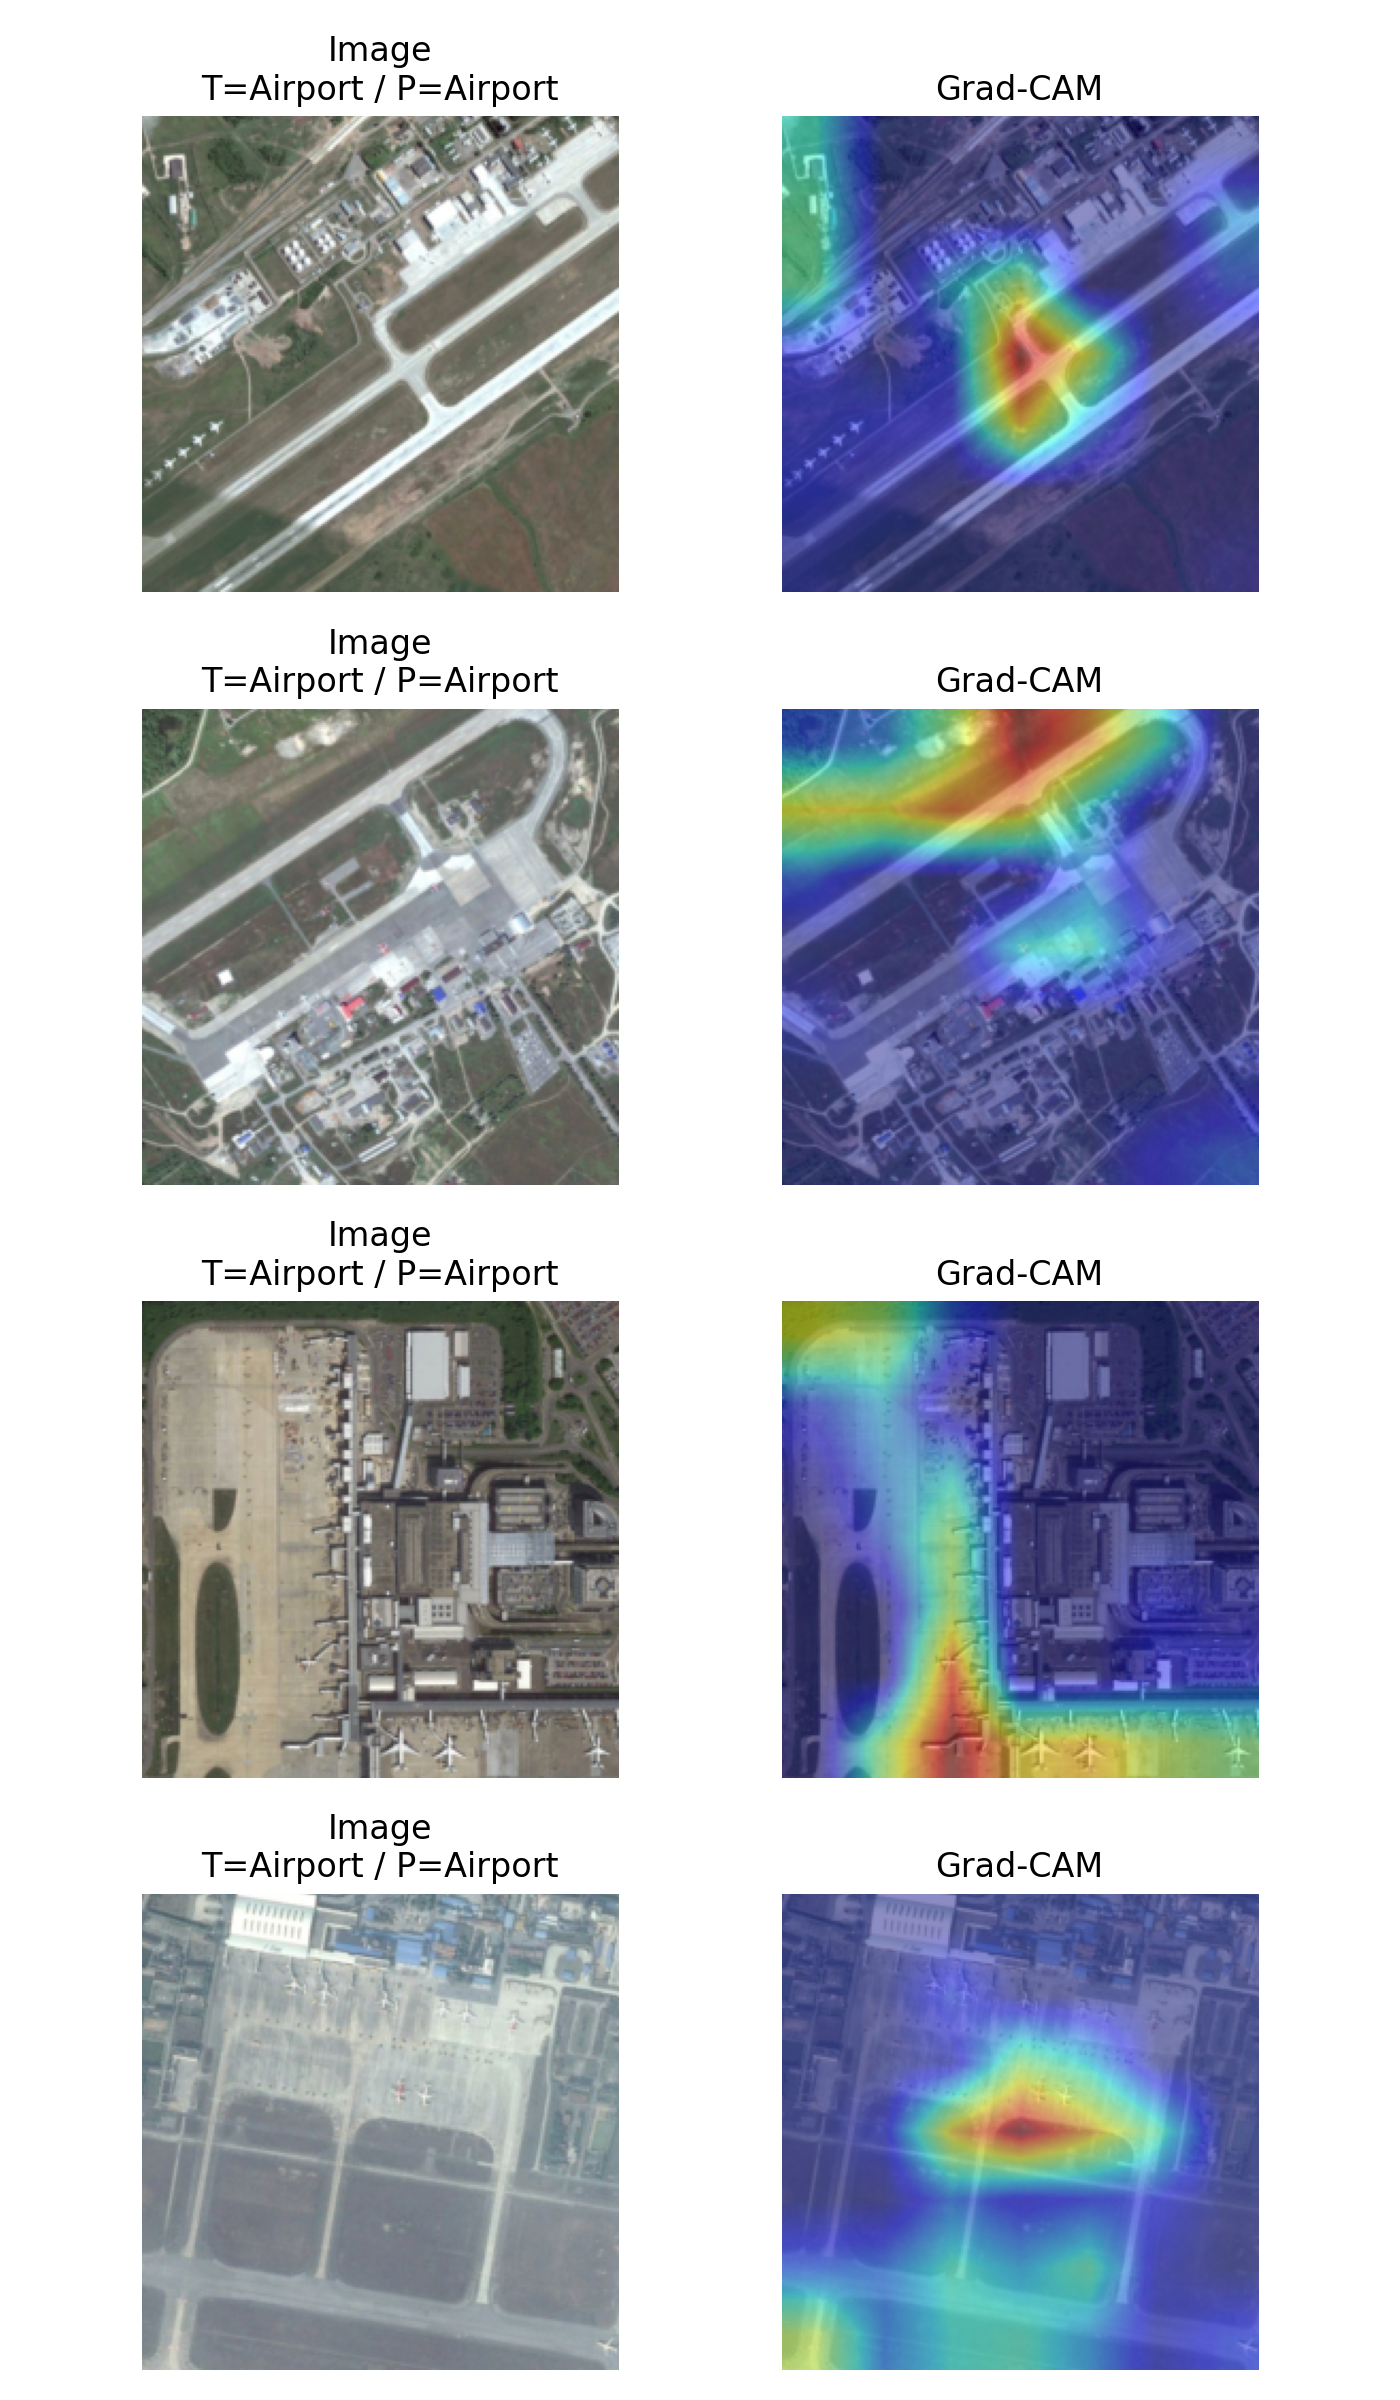
\includegraphics[width=\linewidth]{figures/aid_low20_baseline_activation.png}
    \par\small (a) ConvNeXt-Tiny baseline
  \end{minipage}\hfill
  \begin{minipage}{0.48\linewidth}
    \centering
    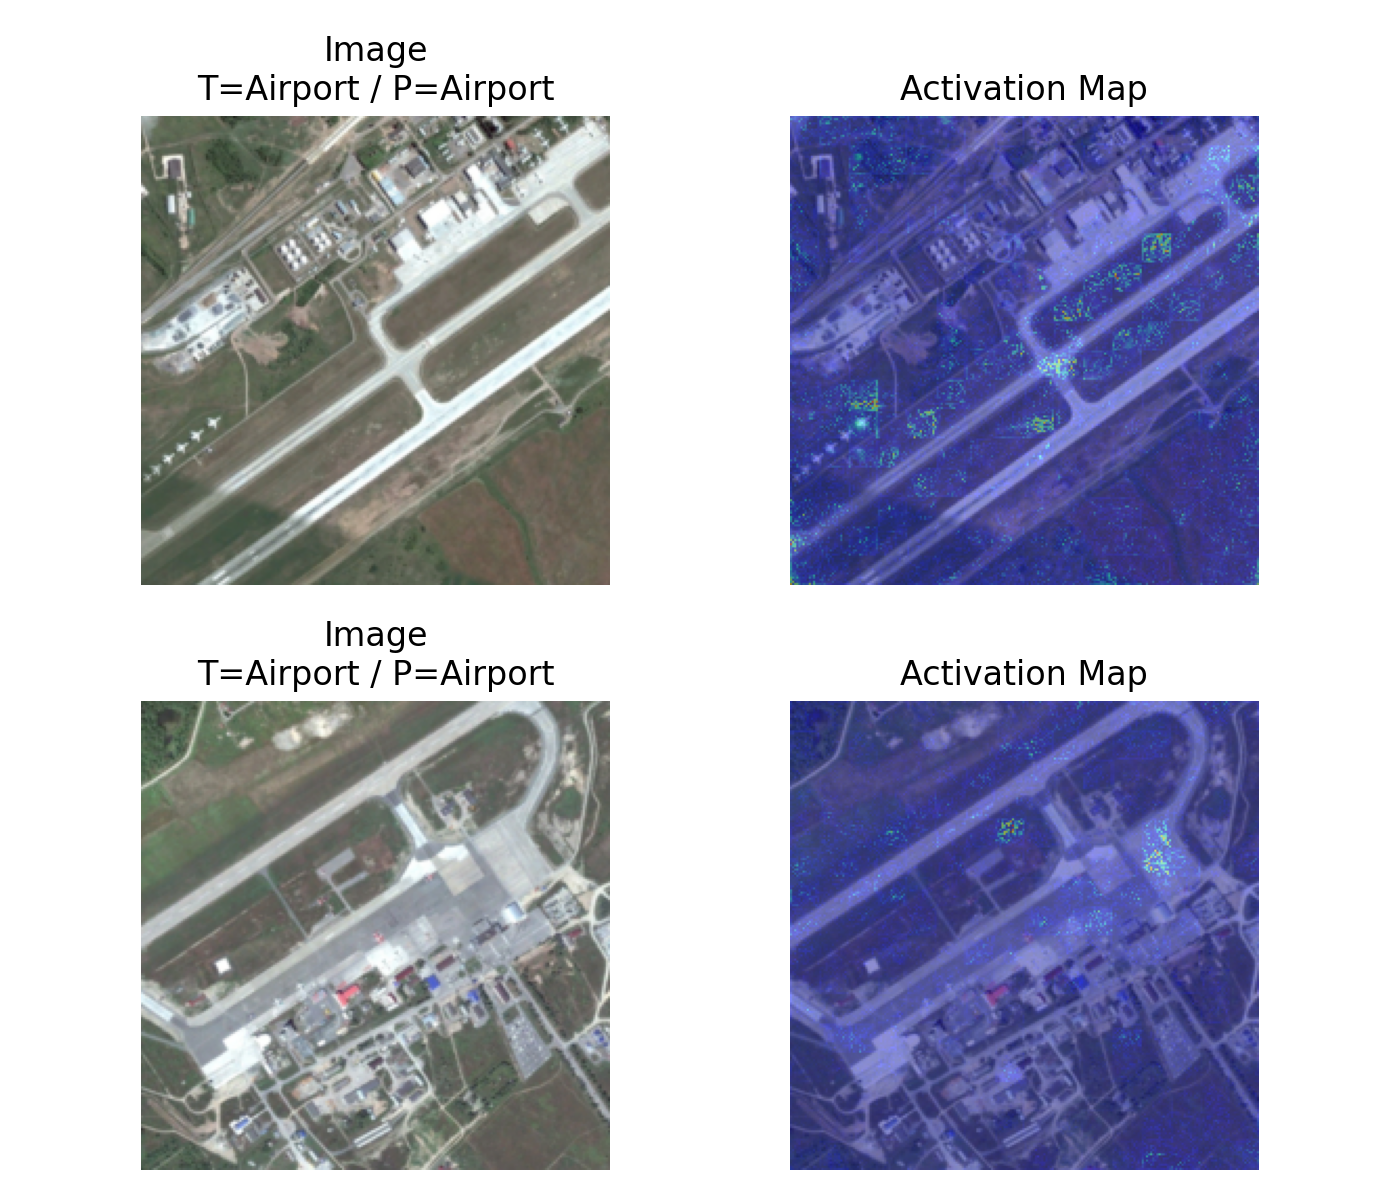
\includegraphics[width=\linewidth]{figures/aid_low20_full_activation.png}
    \par\small (b) Proposed method
  \end{minipage}
  \caption{Gradient-based activation visualizations on AID-low20 from seed 3407. Each pair uses the same test image and the same normalization pipeline for visual comparison.}
  \label{fig:aid_activation}
\end{figure}

\begin{figure}[t]
  \centering
  \begin{minipage}{0.48\linewidth}
    \centering
    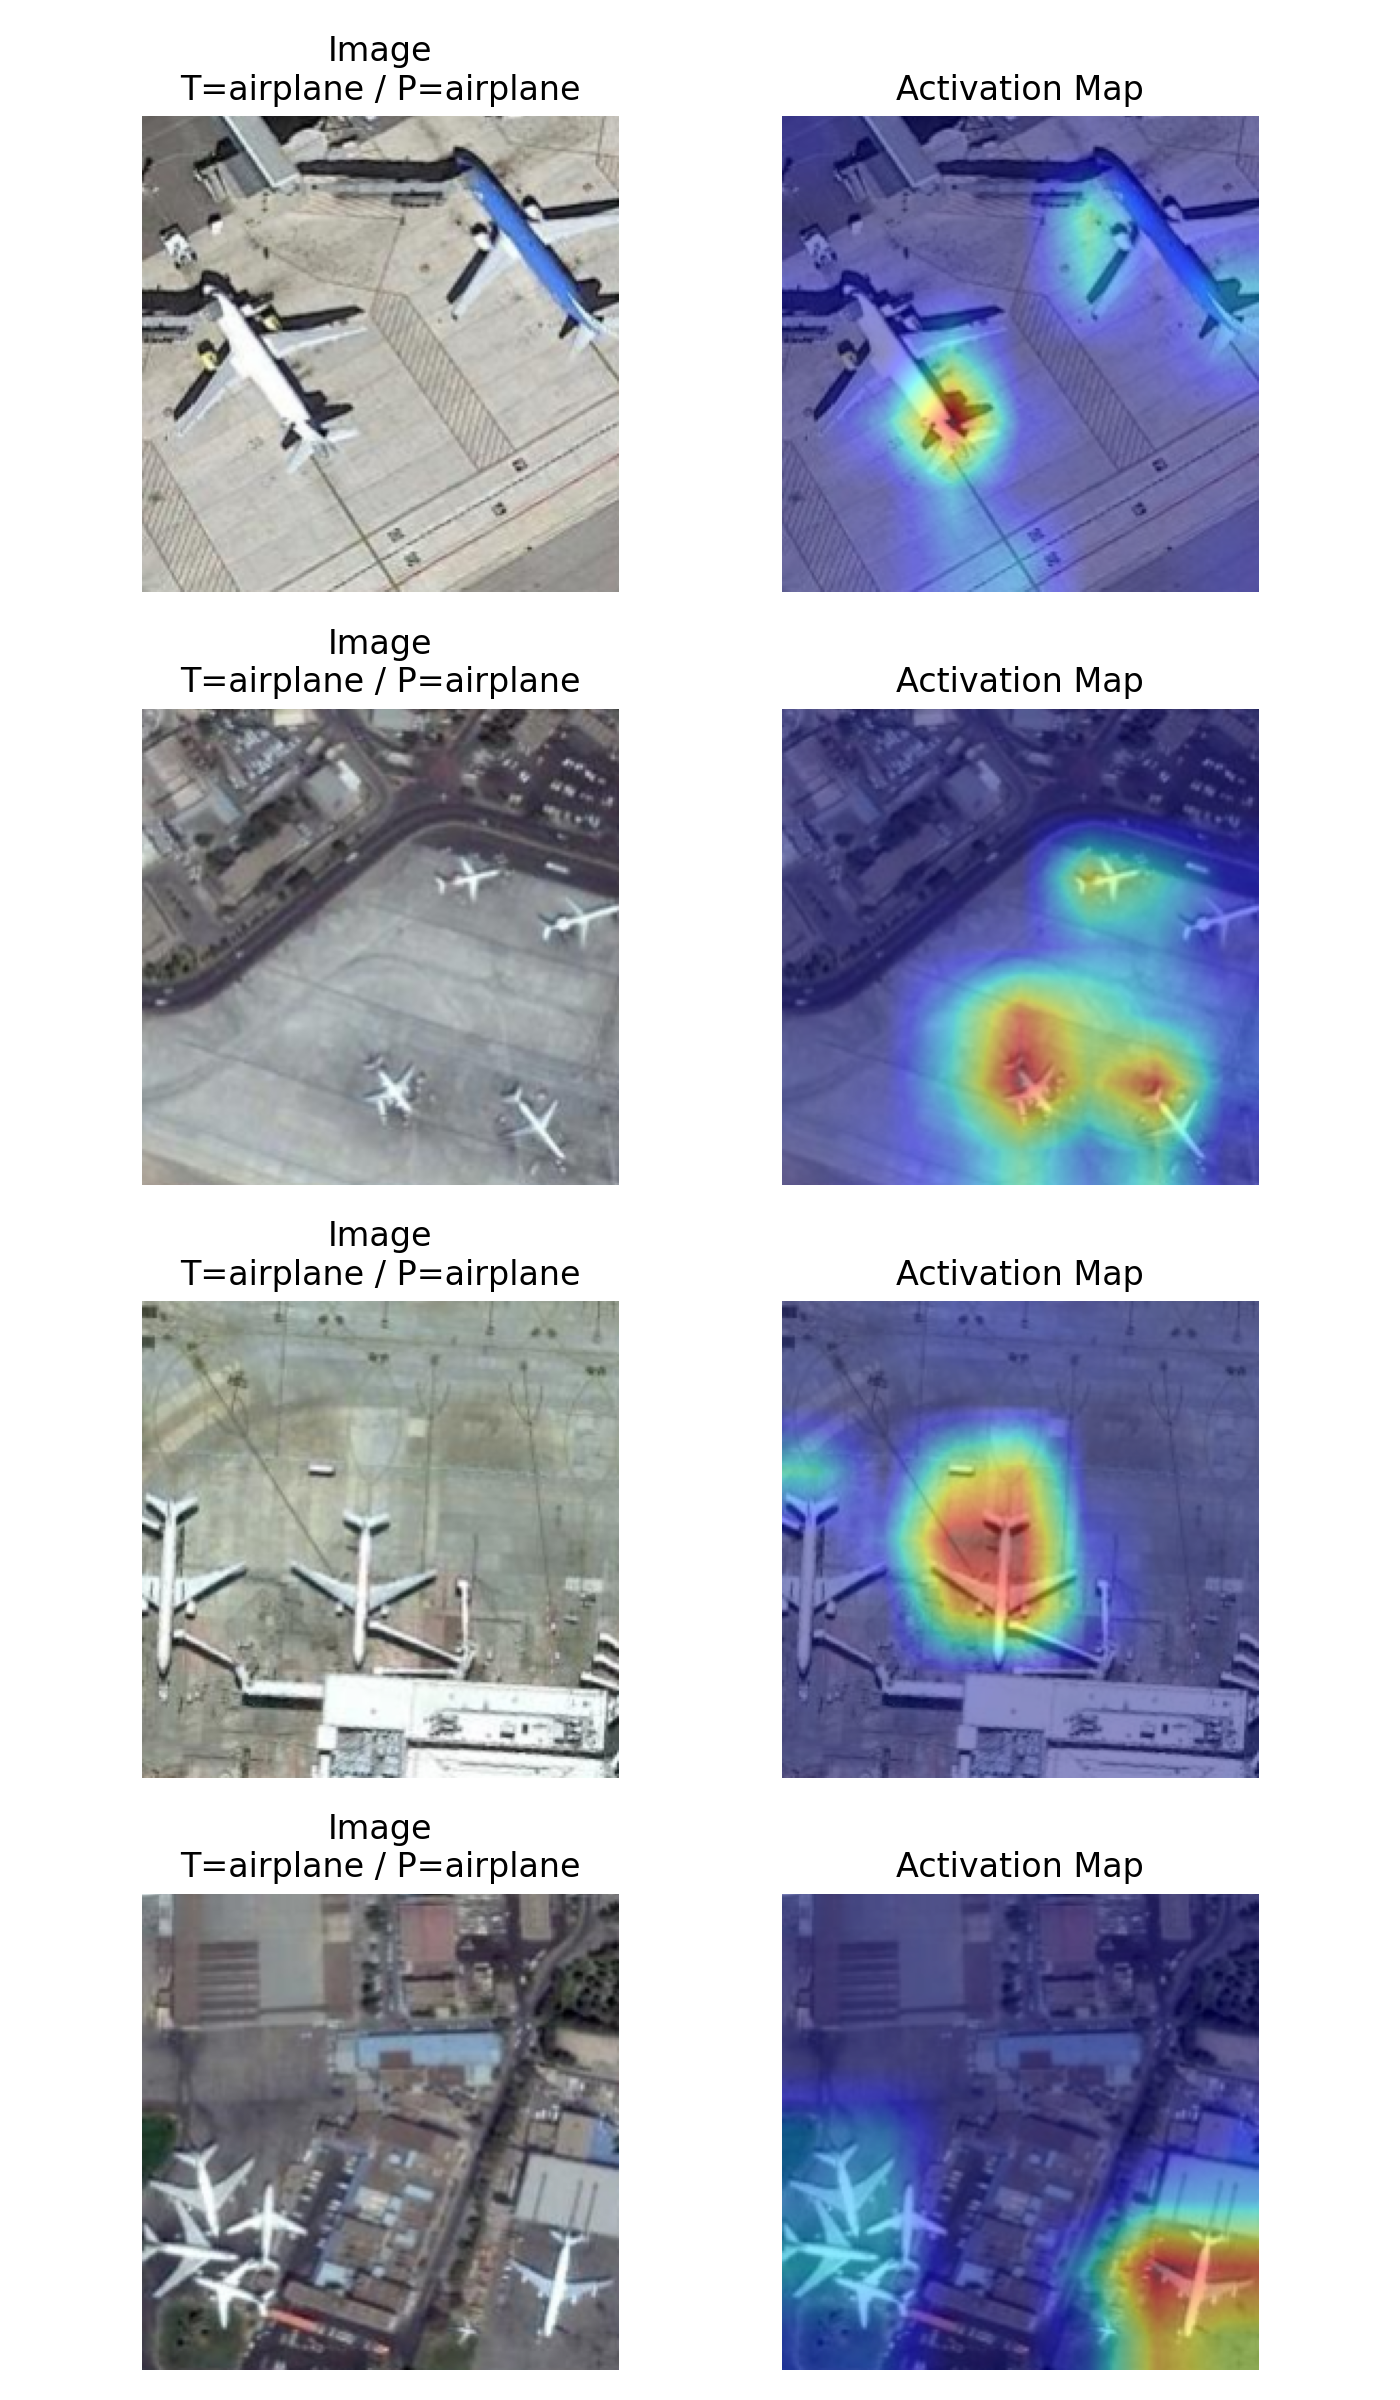
\includegraphics[width=\linewidth]{figures/nwpu_low20_baseline_activation.png}
    \par\small (a) ConvNeXt-Tiny baseline
  \end{minipage}\hfill
  \begin{minipage}{0.48\linewidth}
    \centering
    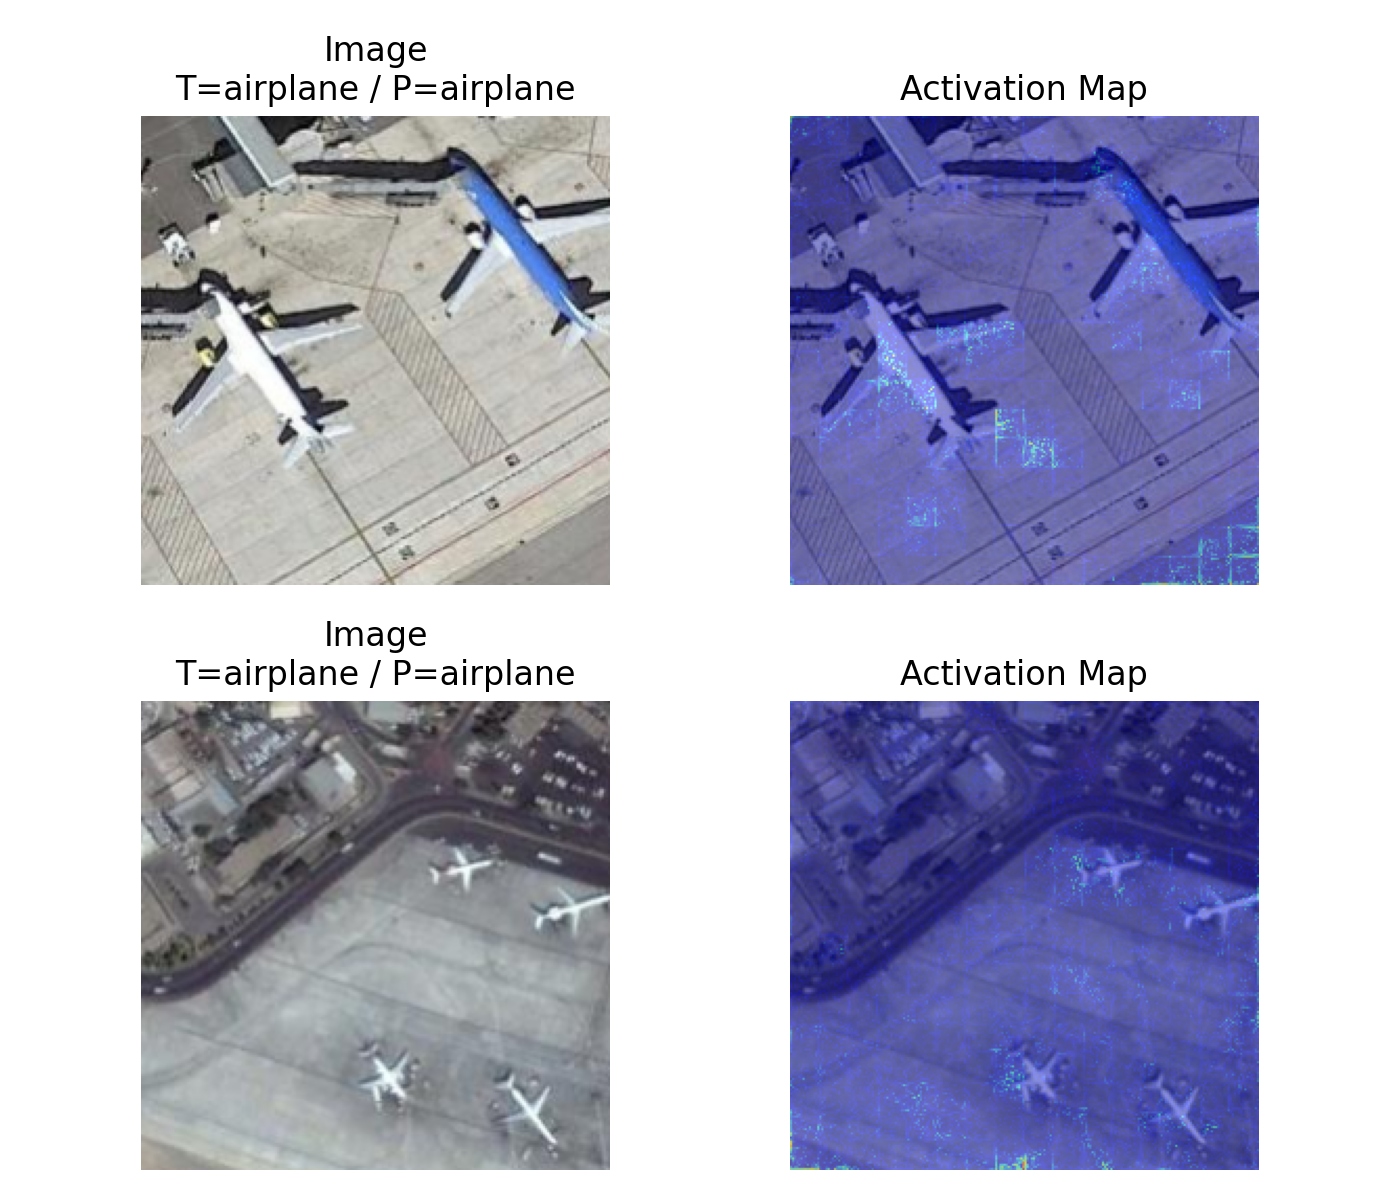
\includegraphics[width=\linewidth]{figures/nwpu_low20_full_activation.png}
    \par\small (b) Proposed method
  \end{minipage}
  \caption{Gradient-based activation visualizations on NWPU-low20 from seed 3407. Each pair uses the same test image and the same normalization pipeline for visual comparison.}
  \label{fig:nwpu_activation}
\end{figure}
